% % ***********************************************************
% ******************* PHYSICS HEADER ************************
% ***********************************************************
% Version 2

\usepackage{amsmath} % AMS Math Package
\usepackage{amsthm} % Theorem Formatting
\usepackage{amssymb}	% Math symbols such as \mathbb
\usepackage{graphicx} % Allows for eps images
\usepackage{multicol} % Allows for multiple columns
\usepackage[dvips,showframe,letterpaper,margin=1.0in,left=1.5in]{geometry}
% tim included
\usepackage[pdftex,bookmarks=true]{hyperref}

\usepackage{cancel}
\usepackage{siunitx}
 % Sets margins and page size
\pagestyle{plain} % Removes page numbers
\makeatletter % Need for anything that contains an @ command 
\renewcommand{\maketitle} % Redefine maketitle to conserve space
{ \begingroup \vskip 10pt \begin{center} \large {\bf \@title}
	\vskip 10pt \large \@author \hskip 20pt \@date \end{center}
  \vskip 10pt \endgroup \setcounter{footnote}{0} }
\makeatother % End of region containing @ commands
\renewcommand{\labelenumi}{(\alph{enumi})} % Use letters for enumerate
% \DeclareMathOperator{\Sample}{Sample}
\let\vaccent=\v % rename builtin command \v{} to \vaccent{}
\renewcommand{\v}[1]{\ensuremath{\mathbf{#1}}} % for vectors
\newcommand{\gv}[1]{\ensuremath{\mbox{\boldmath$ #1 $}}} 
% for vectors of Greek letters
\newcommand{\uv}[1]{\ensuremath{\mathbf{\hat{#1}}}} % for unit vector
\newcommand{\abs}[1]{\left| #1 \right|} % for absolute value
\newcommand{\avg}[1]{\left< #1 \right>} % for average
\let\underdot=\d % rename builtin command \d{} to \underdot{}
\renewcommand{\d}[2]{\frac{d #1}{d #2}} % for derivatives
\newcommand{\dd}[2]{\frac{d^2 #1}{d #2^2}} % for double derivatives
\newcommand{\pd}[2]{\frac{\partial #1}{\partial #2}} 
% for partial derivatives
\newcommand{\pdd}[2]{\frac{\partial^2 #1}{\partial #2^2}} 
% for double partial derivatives
\newcommand{\pdc}[3]{\left( \frac{\partial #1}{\partial #2}
 \right)_{#3}} % for thermodynamic partial derivatives
\newcommand{\ket}[1]{\left| #1 \right>} % for Dirac bras
\newcommand{\bra}[1]{\left< #1 \right|} % for Dirac kets
\newcommand{\braket}[2]{\left< #1 \vphantom{#2} \right|
 \left. #2 \vphantom{#1} \right>} % for Dirac brackets
\newcommand{\matrixel}[3]{\left< #1 \vphantom{#2#3} \right|
 #2 \left| #3 \vphantom{#1#2} \right>} % for Dirac matrix elements
\newcommand{\grad}[1]{\gv{\nabla} #1} % for gradient
\let\divsymb=\div % rename builtin command \div to \divsymb
\renewcommand{\div}[1]{\gv{\nabla} \cdot #1} % for divergence
\newcommand{\curl}[1]{\gv{\nabla} \times #1} % for curl
\let\baraccent=\= % rename builtin command \= to \baraccent
\renewcommand{\=}[1]{\stackrel{#1}{=}} % for putting numbers above =
\newtheorem{prop}{Proposition}
\newtheorem{thm}{Theorem}[section]
\newtheorem{lem}[thm]{Lemma}
\theoremstyle{definition}
\newtheorem{dfn}{Definition}
\theoremstyle{remark}
\newtheorem*{rmk}{Remark}

% ***********************************************************
% ********************** END HEADER *************************
% *********************************************************** 
% \newcommand{\sigdot}[1]{ \gv{\sigma} \hspace{-2pt} \cdot \hspace{-2pt} \v{#1} \,}
% \newcommand{\sigdotg}[1]{ \gv{\sigma} \hspace{-2pt} \cdot \hspace{-2pt} \gv{#1} \,}
% \newcommand{\dotprod}[2]{ \v{#1} \hspace{-2pt} \cdot \hspace{-2pt} \v{#2} \,}

%\newcommand{\beqa}{\begin{eqnarray*} }
%\newcommand{\eeqa}{\end{eqnarray*} }

% \newcommand{\diracdelta}[1]{ \delta^{(3)}(#1) }
% \newcommand{\omin}[1]{ \W_{#1}(p) }
% \newcommand{\omout}[1]{ \W^*_{#1}(p') }
% 
% \newcommand{\E}[1]{ \sqrt{ m^2 + \v{#1}^2 } }
% \newcommand{\E}[1]{ E_{#1} }
% \newcommand{\A}{a}
% \newcommand{\Adag}{a'}
% \newcommand{\qp}{q^{(+)}{}}
% \newcommand{\qm}{q^{(-)}{}}
% 
% \newcommand{\smalldot}{\cdot}
% 
% \newcommand{\gradE}{\grad}
% 
% 
% \newcommand{\snote}[1]{ \small {\bf Sign note:} \emph{ #1} \normalsize }
\chapter{Diagrammatic approach to spin-one particles}

\section{Vertices in the relativistic theory}



The Lagrangian for our relativistic spin-1 theory is
\[
\mathcal{L} 
	=	-\frac{1}{2} (D^\mu W^\nu - D^\nu W^\mu)^\dagger  (D_\mu W_\nu - D_\nu W_\mu) 
				+ m_w^2 W^\dagger W 
				+ i e  [g-1]{W^\dagger}^\mu W^\nu F_{\mu \nu}	
\]


Here $F_{\mu\nu} = \partial_\mu A_\nu - \partial_\nu A_\mu$ is the usual electromagnetic field tensor, and $D = \partial^\mu + i e A^\mu $ is the long derivative.

We have vertices with either one or two photons.  We can get the diagrams by just looking at the Lagrangian.

The one photon terms, involving one power of $A$ are
\[
\mathcal{L}_{A}
	= -\frac{ie}{2} (A^\mu W^\nu - A^\nu W^\mu)^\dagger  (D_\mu W_\nu - D_\nu W_\mu)  
		-\frac{ie}{2} (D^\mu W^\nu - D^\nu W^\mu)^\dagger  (A_\mu W_\nu - A_\nu W_\mu)  
		+  i e [g-2] {W^\dagger}^\mu W^\nu F_{\mu \nu}
\]
So the diagram is

\mbox{
\begin{minipage}{1.6in}
   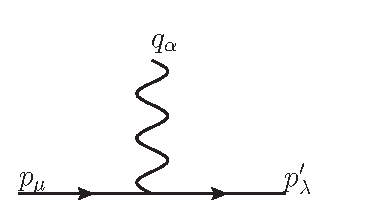
\includegraphics[scale=0.7]{eps/one-photon-fundamental} 
\end{minipage}
$ =  -ie[ g^{\mu\lambda}(p + p')^\alpha - g^{\lambda \alpha} (p' + [g-1]q)^\mu - g^{\alpha \mu} (p - [g-1]q)^\lambda ] $
}

\vspace{2em}


If we write down only the two photon terms:
\[
\mathcal{L}_{A^2 } = \frac{e^2}{2} (A^\mu W^\nu - A^\nu W^\mu)^\dagger  (A_\mu W_\nu - A_\nu W_\mu) 
\]
\[
	= \frac{e^2}{2} \{ 2(W^\dagger \cdot W) (A^\dagger \cdot A)  - 2(W^\dagger \cdot A )(A^\dagger \cdot W) \}
\]

For the two-photon vertex, the term in the Lagrangian can be contracted two ways with the external photon field, so we find:

\mbox{
\begin{minipage}{1.6in}
   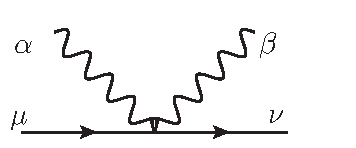
\includegraphics[scale=0.8]{eps/two-photon-fundamental} 
\end{minipage}
$	=	 -i e^2 ( 2 g^{\mu\nu} g^{\alpha \beta} - g^{\mu \beta} g^{\nu \alpha} - g^{\nu\beta}g^{\mu\alpha}) $
}

\section{Wave Functions}

We can relate the Shrodinger-like spinors in the nonrelativistic theory to the relativistic spinors because we can write down the current density in terms of each, and then demand equality:
\[
	\phi^\dagger \phi = j_0
\]
We obtain the relativistic four-current from the Lagrangian.
\subsection{Current in relativistic theory}
We want the conserved current corresponding to the transformation $ W_i \to e^{i \alpha}W_i $, which in infinitesimal form is:
\begin{equation*}
	W_\mu \to W_\mu + i \alpha W_\mu, \;
	W_\mu^\dagger \to W_\mu^\dagger - i \alpha W_\mu^{\dagger}
\end{equation*}

The 4-current density will be:
\begin{equation*}
j^{\sigma} = -i \pd {\mathcal{L} }{W_{\mu, \sigma}} W_\mu  +  i\pd {\mathcal{L} }{W^\dagger_{\mu, \sigma}} W^\dagger_\mu
\end{equation*}

Only one term contains derivatives of the field:

\begin{eqnarray*}
 \pd {\mathcal{L} }{W_{\alpha, \sigma}} 
		&=& \pd{}{W_{\alpha, \sigma}} \left \{ - \frac{1}{2} (D_\mu W_\nu - D_\nu W_\mu)^\dagger(D^\mu W^\nu - D^\nu W^\mu) \right \}\\
		&=& - \frac{1}{2} (D_\mu W_\nu - D_\nu W_\mu)^\dagger (g_{\sigma \mu} g_{\alpha \nu} - g_{\sigma \nu}g_{\alpha \mu})\\
		&=& - (D_\alpha W_\sigma - D_\sigma W_\alpha)^\dagger
\end{eqnarray*}
Likewise:
\begin{eqnarray*}
	\pd {\mathcal{L} }{W_{\alpha, \sigma}^\dagger} 
		&=& - (D_\alpha W_\sigma - D_\sigma W_\alpha)
\end{eqnarray*}
So the four current is

\[
j_\mu = i (\partial_\mu W_\nu - \partial_\nu W_\mu)^\dagger W^{\nu} - i (\partial_\mu W_\nu - \partial_\nu W_\mu) {W^{\dagger}}^\nu 
\]


\subsection{Relation between $\gv{\W}$ and $\phi$}
In the relativistic theory, the scattering amplitudes will involve the polarisations $\W$ of the charged particles.  In the NRQED theory, the amplitudes will involve the spinors $\phi$.  Since each have three degrees of freedom, it is entirely reasonable to expect a direct connection between them.  We can find this relation by calculating the current density in both theories.



Now we write down the current density in the case of $q=0$.  We use that $\partial^\dagger = - \partial$


\beqa
j_0
	&=& i\left\{	(\partial_0 W_\nu - \partial_\nu W_0)^\dagger W^{\nu} -  (\partial_0 W_\nu - \partial_\nu W_0) {W^{\dagger}}^\nu \right \}	\\
	&=& i\left\{	(\partial_0 W_i - \partial_i W_0)^\dagger W^{i} -  (\partial_0 W_i - \partial_i W_0) {W^{\dagger}}^i \right \}	\\
	&=& i\left \{  W^\dagger_i \partial_0^\dagger W^i - W^\dagger_0 \partial_i^\dagger W^{i} - {W^{\dagger}}^i \partial_0 W_i +{ W^{\dagger}}^i \partial_i W_0 \right \}	\\
	&=& i\left \{ -  W^\dagger_i \partial_0 W^i + W^\dagger_0 \partial_i W^{i}- {W^{\dagger}}^i \partial_0 W_i +{ W^{\dagger}}^i \partial_i W_0 \right \}	\\
	&=& i\left \{ - 2 W^\dagger_i \partial_0 W^i + W^\dagger_0 \partial_i  W^{i}+{ W^{\dagger}}^i \partial_i W_0 \right \}	\\
\eeqa


If we write this in terms of charged particle polarisations $\W$ and momentum $p$ we get
\[
j_0(p) = 	- 2 \W^\dagger_i p_0 \W^i + \W^\dagger_0 p_i \W^{i} +{ \W^{\dagger}}^i p_i \W_0
\]
\[
	=	+ 2 p_0 \gv{\W}^\dagger \cdot \gv{\W} - \W^\dagger_0 \v{p} \cdot \gv{\W} - \gv{\W}^\dagger \cdot \v{p} \W_0
\]
Then using that $\W_0 = \frac{\gv{\W} \cdot \v{p}}{p_0}$
\[
	j_0 = 2 p_0 \gv{\W}^\dagger \cdot \gv{\W} - 2 \frac{ ( \gv{\W}^\dagger \cdot \v{p})( \v{p} \cdot \gv{\W} )}{p_0} 
\]

Here we want to write the current as a set of operators between the polarisations $\W_i$. Since the above connects different components of the polarisation, this will necessitate using spin matrices $\v{S}$.  In the appendix I derive the necessary identity.  Using that, we get
\[
	j_0 = 2p_0 \W^\dagger_i \left\{ \delta_{ij} - \frac{ \v{p}^2 \delta_{ij} - (\v{S} \cdot \v{p})^2_{ij} }{p_0^2} \right \} \W_j
\]
Then by demanding $j_0 = \phi^\dagger \phi$ we can get a relation between $\phi$ and $\gv{\W}$.
\[
 2p_0 \W^\dagger_i \left\{ \delta_{ij} - \frac{ \v{p}^2 \delta_{ij} - (\v{S} \cdot \v{p})^2_{ij} }{p_0^2} \right \} \W_j = \phi^\dagger \phi
\]
\[
	\gv{\W}  = \left\{ 2p_0 \left (1 - \frac{ \v{p}^2 - (\v{S} \cdot \v{p})^2 }{p_0^2}   \right ) \right \}^{-\frac{1}{2}} \phi
\]
To the order needed, this is
\[
	\gv{\W} = \frac{1}{\sqrt{2p_0}} \left (1 + \frac{ \v{p}^2 - (\v{S} \cdot \v{p})^2 }{2m^2} \right ) \phi
\]
\[
	=	 \frac{1}{\sqrt{2m}} \left (1 + \frac{ \v{p}^2}{4m^2} - \frac{(\v{S} \cdot \v{p})^2 }{2m^2} \right ) \phi
\]


\section{One Photon Calculation}


First we do the calculations necessary to fix the one-photon terms in the NRQED Lagrangian.  We consider the process of a single charged particle scattering off an external field, and calculate the amplitude in the relativistic theory.  



We already have the one photon diagram, for incoming momentum $p$, outgoing $p'$ and photon momentum $q$ (so that $p' = p + q$).  
\[	ie\left[ g^{\mu\nu} (p + p')^\lambda - g^{\nu\lambda}([g-1] q+p')^\mu + g^{\lambda\mu}([g-1] q-p)^\nu \right] \]

Contracted with external polarizations $\omin{\mu}$, $\omout{\nu}$ and external field $A_\lambda(q)$, this becomes
\[
	ie\ \omin{\mu} \omout{\nu} \left[ g^{\mu\nu} (p + p')\cdot A - A^\nu ( [g-1] q+p')^\mu + A^\mu ( [g-1] q-p)^\nu \right]
\]

The W polarizations are subject to the condition that $ k \cdot \W(k) = 0 $.  We can use that to simplify the above, since then $p'^\mu \omin{\mu} = q^\mu \omin{\mu}$ and $p^\nu \omout{\nu} = -q^\nu \omout{\nu}$.  So the vertex becomes

\[
	ie\ \omin{\mu} \omout{\nu} \left[ g^{\mu\nu} (p + p')\cdot A  +g ( q^\nu A^\mu - q^\mu A^\nu ) \right] 	
\]

There are two terms here, one proportional to $g$ and one that has no $g$ dependence.  The first term is
\[
	ie\ \omin{\mu} \omout{\nu} g^{\mu\nu} (p + p')\cdot A 
\]
while the second is 
\[
	ie\ \omin{\mu} \omout{\nu} [g] ( q^\nu A^\mu - q^\mu A^\nu ) 	
\]


%%% G independant one-photon terms
\subsection{First term (no $g$ dependence)}

We've written the vertex such that there are two terms:   Our strategy for each will be the same: first write in terms of a matrix element between $\phi^\dagger \phi$, and then Fourier transform to write results in terms of external fields $\v{B}$ and $\v{E}$.


We first expand in terms of $\W_i$ and then use the spin identity to put in the form of a matrix element.

The first term is 
\beqa
ie \omin{\mu} \omout{\nu}  g^{\mu\nu} (p + p')\cdot A
	&=& 	ie (p + p')\cdot A ( \omin{0} \omout{0} - \omin{i} \omin{i})	\\
	&=&	ie [(p + p')\cdot A] \omout{j} \left( \frac{p'_j p_i}{p_0^2} - \delta_{ij} \right) \omin{i}	\\
	&=&	ie [(p + p')\cdot A] \gv{\W}^\dagger (p')  \left(  
			\frac{ \v{p} \cdot \v{p}' - (\v{S} \cdot \v{p})( \v{S} \cdot \v{p}') }{p_0^2}  -1 \right) \gv{\W}(p)
\eeqa
(We assume that $q_0=0$, so $p'_0 = p_0$.)

In terms of the wave functions $\phi$ this becomes
\[
	-ie \frac{(p + p')\cdot A}{2p_0} \phi^\dagger
		\left( 1 + \frac{\v{p'}^2 - (\v{S}\cdot \v{p'})^2 }{2m^2} \right) 
		\left(1 - \frac{ \v{p} \cdot \v{p}' - (\v{S} \cdot \v{p})( \v{S} \cdot \v{p}')}{m^2} \right)
		\left( 1 + \frac{\v{p}^2 - (\v{S}\cdot \v{p})^2 }{2m^2} \right)
	\phi
\]

Simplifying to the order needed
\[
	-ie \frac{(p + p')\cdot A}{2p_0} \phi^\dagger
		\left( 1  + \frac{1}{2m^2} \left \{ \v{q} \cdot \v{p}' - (\v{S} \cdot \v{q})( \v{S} \cdot \v{p'})
			- \v{p} \cdot \v{q} + (\v{S} \cdot \v{p})( \v{S} \cdot \v{q}) \right \} \right )	
	\phi
\]
\[
	= -ie \frac{(p + p')\cdot A}{2p_0} \phi^\dagger
		\left( 1  + \frac{1}{2m^2} \left \{ \v{q}^2 + [\v{S} \cdot \v{p}, \v{S} \cdot \v{q}] - (\v{S} \cdot \v{q})^2 \right \}
	 \right )\phi
\]
\[
	= -ie \frac{(p + p')\cdot A}{2p_0} \phi^\dagger
		\left( 1  + \frac{1}{2m^2} \left \{ \v{q}^2 + i \v{S} \cdot \v{p} \times \v{q} - (\v{S} \cdot \v{q})^2 \right \}
	 \right )\phi
\]

Expanding the outside term, (again using $p'_0 = p_0$)
\[
	\frac{(p + p')\cdot A}{2p_0} = \frac{2p_0}{2p_0} A_0 - \frac{(\v{p} + \v{p'})\cdot \v{A} }{2p_0}
		= A_0 -  \frac{(\v{p} + \v{p'})\cdot \v{A} }{2p_0}
\]


We can simplify 
\[
	-ie  \phi^\dagger(p') \left( A_0  + \frac{A_0}{2m^2}( \v{q}^2 + i \v{S} \cdot \v{p} \times \v{q} - (\v{S} \cdot \v{q})^2 )
	- \frac{(\v{p} + \v{p'})\cdot \v{A} }{2p_0}
	- \frac{(\v{p} + \v{p'})\cdot \v{A} }{2m} \frac{i \v{S} \cdot \v{p} \times \v{q}}{2m^2} \right ) \phi(p)
\]

Remember that we want to write this in terms the external field and its derivatives in position space.  So we Fourier transform such that the transferred momentum $\v{q}$ becomes a derivative on the external field.  The prescription is $\v{q} \to -i \grad$.  

%%% A_0 terms
\subsubsection{Higher order terms involving $A_0$}
The second order term involving $A_0$ has both first and second derivatives of the potential.  The electric field is $E_i = -\partial_i A_0$ and so $q_i A_0 \to i E_i$.  Then $q_i q_j A_0 = \partial_j E_i = \partial_i E_j$.  Applying this to the higher order terms coupled to $A_0$:
\[
A_0( \v{q}^2 + i \v{S} \cdot \v{p} \times \v{q} - (\v{S} \cdot \v{q})^2 )
	\to \grad \cdot \v{E} -  \v{S} \cdot \v{p} \times \v{E} - S_i S_j \grad_i E_j 
\]

%%% A_i terms
\subsubsection{Higher order terms involving $\v{A}$}
We need to simplify the final term: $(\v{p} + \v{p'})\cdot \v{A}  (\v{S} \cdot \v{p} \times i\v{q})$.  We first find just $iq_i (\v{p} + \v{p'}) \cdot \v{A}$.  Using $\epsilon_{ijk} B_k = i(q_i A_j - q_j A_i)$ we get
\[
	(p + p')_i \epsilon_{ijk} B_k = (p + p')_i  \left( i q_i A_j - i q_j A_i \right )
\]
Now we use the kinematic fact that we deal with elastic scattering.  Since in this case $ ( \v{p'} + \v{p}) \cdot \v{q} = \v{p'}^2 - \v{p}^2 = 0$, the $(p+p')_i q_i$ term vanishes, leaving
\[
	(p + p')_i \epsilon_{ijk} B_k = -i (p + p')_i q_j A_i = -i q_j(\v{p} + \v{p'}) \cdot \v{A} 
\]

So we have the identity
\[
i q_j (\v{p} + \v{p'}) \cdot \v{A}  =  - \epsilon_{ijk} (p + p')_i  B_k
\]
We use this identity to deal with the more complicated term:
\beqa
(\v{p} + \v{p'}) \cdot \v{A} ( \v{S} \cdot \v{p} \times i\v{q} )
	&=&	 S_i p_j  \epsilon_{ijk} [i q_k (\v{p} + \v{p'}) \cdot \v{A} ]	\\
	&=&	- S_i p_j \epsilon_{ijk} [ \epsilon_{\ell k m} (p + p')_\ell B_ m]	\\
	&=&	 S_i p_j \epsilon_{ijk} [ \epsilon_{\ell m k} (p + p')_\ell B_ m]	\\
	&=&	S_i p_j (p+p')_\ell B_m [\delta_{i \ell} \delta_{jm} - \delta_{i m} \delta_{j \ell}]	\\
	&=&	\v{S} \cdot  (\v{p} + \v{p'}) \v{B} \cdot \v{p} - \v{S} \cdot \v{B} (\v{p} + \v{p'}) \cdot \v{p} \\
\eeqa
For the case of a constant $\v{B}$, any terms of the type $q_i B_j$ vanish.  So the above reduces to
\[
(\v{p} + \v{p'}) \cdot \v{A}  (\v{S} \cdot \v{p} \times i\v{q} )
	= 2 \{  (\v{S} \cdot  \v{p})( \v{B} \cdot \v{p}) - \v{p}^2 \v{S} \cdot \v{B} \}
\]


%%% Total one-photon g-independant terms
\subsubsection{Total contribution of the $g$-independent term} 

So the first term in the vertex produces the following contribution to the scattering amplitude.
\[ie \omin{\mu} \omout{\nu}  g^{\mu\nu} (p + p')\cdot A \to \]
\[
	 -ie \phi^\dagger(p') \left( A_0  + \frac{1}{2m^2}( \grad \cdot \v{E} -  \v{S} \cdot \v{p} \times \v{E} - S_i S_j \grad_i E_j )
	- \frac{\v{p}\cdot \v{A} }{p_0}
	+ \frac{1}{2m^3}\{ \v{p}^2 \v{S} \cdot \v{B} -  (\v{S} \cdot  \v{p})( \v{B} \cdot \v{p}) \} \right )\phi(p)
\]


\subsection{Second term (proportional to $g$)}
The second term looks like the external polarisations contracted with something like $F_{\mu\nu}$:
\[
	ie\ \omin{\mu} \omout{\nu} [g] ( q^\nu A^\mu - q^\mu A^\nu ) 	
\]
\subsubsection{General tensor type term}
Before calculating the specific term in question, we can consider the general type of term $\omout{\nu} \omin{\mu} u^\nu v^\mu$.  We want to express it as a matrix element between the vector part of the polarization. 

\beqa
\omout{\nu} \omin{\mu} u^\nu v^\mu
	&=&	\W_0'  u_0 v_0 \W_0
		- (\v{\W}' \cdot \v{u}) v_0 \W_0
		- \W_0' u_0 (\v{v} \cdot \gv{\W}) 
		+ (\gv{\W'} \cdot \v{u})( \v{v} \cdot \gv{\W})	\\
	&=&	\frac{ \gv{\W'} \cdot \v{p'} u_0}{p'_0} \frac{ \gv{\W} \cdot \v{p} v_0}{p_0}
		- (\v{\W}' \cdot \v{u}) \frac{ \gv{\W} \cdot \v{p} v_0}{p_0}
		- \frac{ \gv{\W'} \cdot \v{p'} u_0}{p'_0}  (\v{v} \cdot \gv{\W}) 
		+ (\gv{\W'} \cdot \v{u})( \v{v} \cdot \gv{\W})	\\
	&=&	\gv{\W}'_j \left (
			\frac{ u_0 v_0}{p_0 p'_0} p'_j p_i
			- \frac{v_0}{p_0} u_j p_i
			- \frac{u_0}{p'_0} p'_j v_i
			+ u_j v_i
		\right ) \W_i	\\
	&=&	\gv{\W'}^\dagger \left (
			\frac{ u_0 v_0}{p_0 p'_0} [ \v{p} \cdot \v{p'} - (\v{p} \cdot \v{S}) (\v{p'} \cdot \v{S}) ]
			- \frac{v_0}{p_0} [ \v{p} \cdot \v{u} - (\v{p} \cdot \v{S}) (\v{u} \cdot \v{S}) ] \right.
	\\&&		\left. - \frac{u_0}{p'_0} [ \v{v} \cdot \v{p'} - (\v{v} \cdot \v{S}) (\v{p'} \cdot \v{S}) ]
			+ [ \v{v} \cdot \v{u} - (\v{v} \cdot \v{S}) (\v{u} \cdot \v{S}) ]
		\right ) \gv{\W}	\\
\eeqa

\subsubsection{$F_{\mu\nu}$ term}

Now we use that identity to express the term that's like $\W'_\nu \W_\mu F^{\mu\nu}$, with $q_0=0$ (and thus $p'_0 = p_0)$.

\beqa
+ie g \W'_\nu \W_\mu (q^\nu A^\mu - q^\mu A^\nu)
	&=&	+ie g\gv{\W'}^\dagger \Bigg(
			-\frac{A_0}{p_0} \left\{ \v{p} \cdot \v{q} - (\v{p} \cdot \v{S}) (\v{q} \cdot \v{S}) \right\}
			+ \frac{A_0}{p_0} \left\{ \v{q} \cdot \v{p'} - (\v{q} \cdot \v{S}) (\v{p'} \cdot \v{S}) \right\}
	\\&&		+\left\{ \v{q} \cdot \v{A} - (\v{A} \cdot \v{S}) (\v{q} \cdot \v{S}) \right\}
			-\left\{ \v{A} \cdot \v{q} - (\v{q} \cdot \v{S}) (\v{A} \cdot \v{S}) \right\}
		\Bigg) \gv{\W}	\\
	&=&	+ie g\gv{\W'}^\dagger \left\{
			\frac{A_0}{p_0} \Big( \v{q}^2 - (\v{q} \cdot \v{S} )^2 + [\v{p} \cdot \v{S}, \v{q} \cdot \v{S}] \Big)
			- [\v{A} \cdot \v{S}, \v{q} \cdot \v{S}]
		\right\} \gv{\W}
\eeqa

Now we express the polarization vectors in terms of the spinor $\phi$.  The first term above has $A_0$, the second $\v{A}$.

%%% A_0 terms
\subsubsection{$A_0$ terms}
The first term coupled to $A_0$ is already second order, so we can just use $\v{\W} \to \frac{1}{\sqrt{2m}}\phi$
\[
	ie g\phi^\dagger(\v{p'})   \frac{A_0}{2m^2} \left( \v{q}^2 - (\v{q} \cdot \v{S} )^2 + i\v{S} \cdot \v{p} \times \v{q} \right) \phi (\v{p})
\]
This is exactly the same structure that arose in the previous term, that which had no dependence on $g$.  In terms of E it is
\[
 ie g \frac{1}{2m^2}\phi^\dagger(\v{p'})  ( \grad \cdot \v{E} -  \v{S} \cdot \v{p} \times \v{E} - S_i S_j \grad_i E_j ) \phi (\v{p})
\]

%%% A_i terms
\subsubsection{$\v{A}$ terms}
The second term  is  $-ie g\gv{\W^\dagger} [\v{A} \cdot \v{S}, \v{q} \cdot \v{S}] \gv{\W}$.  The commutator is:
\beqa
[\v{A} \cdot \v{S}, \v{q} \cdot \v{S}]
	&=&	A_i q_j [S_i, S_j]	\\
	&=&	A_i q_j (i\epsilon_{ijk} S_k)	\\
	&=&	- \v{S} \cdot i\v{q} \times \v{A}	\\
	&\to&	- \v{S} \cdot \grad \times \v{A} 	\\
	&=&	-\v{S} \cdot \v{B}	\\
\eeqa
So the whole thing is $ieg \gv{\W^\dagger} (\v{S} \cdot \v{B}) \gv{\W}$, which is first order, so we need corrections to this term coming from the expression for $\W$ in terms of $\phi$.

\[
 ieg\gv{\W^\dagger} (\v{S} \cdot \v{B}) \gv{\W} \to
	ieg \frac{1}{2p_0} \phi^\dagger
		\left( 1 + \frac{\v{p'}^2 - [\v{S}\cdot \v{p'}]^2 }{2m^2} \right) 
		\v{S} \cdot \v{B}
		\left( 1 + \frac{\v{p}^2 - [\v{S}\cdot \v{p}]^2 }{2m^2} \right)
	\phi
\]


Since we deal with a constant $B$ field, all terms with $q$ vanish, so the above is really
\[
	=  ieg \frac{1}{2p_0} \phi^\dagger	\left(  
		\v{S} \cdot \v{B} +  \v{S} \cdot \v{B} \frac{p^2}{2m^2} + \frac{1}{2m^2}\left\{ \v{S} \cdot \v{B}, \frac{\v{p}^2}{2} - [\v{S}\cdot \v{p}]^2 \right\}_+	\right ) \phi
\]
Expanding $\frac{1}{2p_0} = \frac{1}{2m}(1 - \frac{\v{p}^2}{2m^2} )$ eliminates the second term:
\[
	=  ieg \frac{1}{2m} \phi^\dagger	\left(  
		\v{S} \cdot \v{B}  + \frac{1}{2m^2}\left\{ \v{S} \cdot \v{B}, \frac{\v{p}^2}{2} - [\v{S}\cdot \v{p}]^2 \right\}_+	\right ) \phi
\]



From the earlier spin-1 work we actually have an identity for the anticommutator, the derivation of which I attach as an appendix:
\[
\left \{ \frac{\v{p}^2}{2} - (\v{S} \cdot \v{p})^2, \v{S} \cdot \v{B} \right \} = -\frac{(\v{S} \cdot \v{p})( \v{B} \cdot \v{p})}{2m^2}
\]
Using that, we find that the term finally reduces to
\[
	ieg \frac{1}{2m}\phi^\dagger \left( \v{S} \cdot \v{B} - \frac{(\v{S} \cdot \v{p})( \v{B} \cdot \v{p})}{2m^2}  \right) \phi
\]

\subsubsection{Total contribution of one-photon $g$ dependent terms}
We can now write the total contribution of the second $g$-dependent term to the scattering amplitude.
\[
ieg \frac{1}{2m}\phi^\dagger \left ( \v{S} \cdot \v{B} - \frac{(\v{S} \cdot \v{p})( \v{B} \cdot \v{p})}{2m^2}  + \frac{1}{m} \left\{ \grad \cdot \v{E} -  \v{S} \cdot \v{p} \times \v{E} - S_i S_j \grad_i E_j \right \} \right ) \phi
\]



%%%%%%%%% ALL TERMS TOGETHER  %%%%%%%%%%%%%
\subsection{All terms together}
Now that we've expressed each of the terms, we can write down the total scattering amplitude, as calculated in the relativistic theory.  (Elastic scattering off an external field, with constant $\v{B}$.)

First consider the terms related to the electric field/potential:
\[ 
	-ie\phi^\dagger \left( A_0  - (g-1)  \frac{1}{2m^2} \{ \grad \cdot \v{E} -  \v{S} \cdot \v{p} \times \v{E} - S_i S_j \grad_i E_j \} \right) \phi
\]
The terms with bare $\v{A}$:
\[
ie\phi^\dagger \left( \frac{\v{p}\cdot \v{A} }{p_0}\right ) \phi 
	\approx
ie\phi^\dagger \left( \frac{\v{p}\cdot \v{A} }{m} - \frac{\v{p}\cdot \v{A} \v{p}^2}{2m^3}\right ) \phi 
\]

Then the terms with $B$ in them:
\[
	i\frac{e}{2m}\phi^\dagger \left(  
		g \v{S} \cdot \v{B} -  \v{S} \cdot \v{B} \frac{\v{p}^2}{m^2}
		-\frac{g-2}{4m^2}(\v{S} \cdot \v{p} )( \v{B} \cdot \v{p})
	\right ) \phi
\]

So the whole thing is:

\[
iM_{REL} = -ie \phi^\dagger \Big (
		 A_0  - \frac{\v{p}\cdot \v{A} }{m} + \frac{\v{p}\cdot \v{A} \v{p}^2}{2m^3}
		- \frac{g-1}{2m^3}\{ \grad \cdot \v{E} -  \v{S} \cdot \v{p} \times \v{E} - S_i S_j \grad_i E_j \}
		- g\frac{1}{2m} \v{S} \cdot \v{B}
		+ \v{S} \cdot \v{B} \frac{\v{p}^2}{2m^3}
		+ \frac{g-2}{4m^3}(\v{S} \cdot \v{p} )( \v{B} \cdot \v{p})
	\Big ) \phi
\]



\section{Two Photon Calculation}


We want to calculate the coefficients of some two-photon terms in the NRQED Lagrangian from relativistic diagrams, in the spin-1 theory.  We do so by calculating the amplitude for Compton scattering in the relativistic theory.  

There are two types of contributions, one from the fundamental two-photon vertex and the other from combination of two one-photon vertices.  Two-photon contact terms in the Lagrangian will have an additional symmetry factor of 1/2 compared to the expression for the vertex.

\begin{minipage}{1in}
   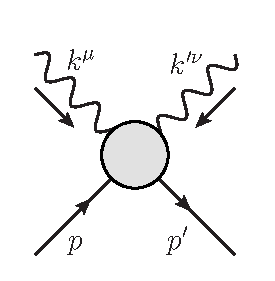
\includegraphics[scale=0.7]{eps/blob1} 
\end{minipage}
$=$
\begin{minipage}{1.6in}
   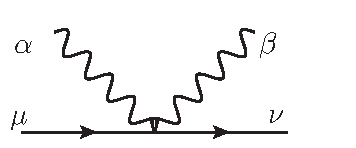
\includegraphics[scale=0.7]{eps/two-photon-fundamental} 
\end{minipage}
$+$
\begin{minipage}{1.6in}
   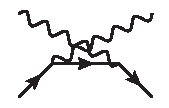
\includegraphics[scale=1]{eps/crossed-small} 
\end{minipage}
$+$
\begin{minipage}{1.6in}
   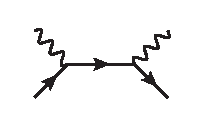
\includegraphics[scale=1]{eps/uncrossed-small} 
\end{minipage}


In this calculation we say the incoming charged particle has momentum $p$, the outgoing, momentum $p'$.  We define both photon momenta $k$ and $k'$ going \emph{into} the vertex or vertices.  Charged particle polarisations are $\W$, while photon polarisations are $\A$.

Once we've calculated the scattering amplitude we need to relate it to the NRQED vertices.  The first step will be to write all terms "sandwiched" between $\W^\dagger$ and $\W$.  Some terms will already be proportional to $\gv{\W^\dagger} \cdot \gv{\W}$.  But there will be others of the form $[\gv{\W^\dagger} \cdot \v{u}] [\v{v} \cdot \gv{\W}]$.  To deal with these we introduce the spin matrices $\v{S}$, and use the identity:
\[
	(\gv{\W^\dagger} \cdot \v{u}) (\v{v} \cdot \gv{\W}) = \W^\dagger_a \left( \delta_{ab} \v{u} \cdot \v{v} - v_i u_j\{S_i S_j\}_{ab}  \right) \W_b
\]


Once written in this form, our recipe will then be to replace photon polarisations $\A$ with the external field $A$.  We choose the gauge where $\A=0$, so the field $\v{E}$ comes from	$ik_0 \A_0(k) \to \v{E}$, while the bare polarisation $\v{\A}(k) \to \v{A}$.

The charged particle polarisations must be replaced by the Schrodinger-like wave functions $\phi$.  Consistent with the calculations for the one-photon terms, the prescription is:
\[
	\gv{\W}(p) \to \frac{1}{\sqrt{2m}}\left( 1 + \frac{\v{p}^2}{4m^2} - \frac{ [\v{S}\cdot \v{p}]^2 } {2m^2} \right)\phi(\v{p})
\]





\section{Two-photon vertex}

%TODO add diagram?
The relativistic two-photon vertex is
\[
 -i e^2 ( 2 g^{\mu\nu} g^{\alpha \beta} - g^{\mu \beta} g^{\nu \alpha} - g^{\mu \alpha} g^{\nu \beta} )
\]
If we contract with the photon and charged particle polarisations, we get
\[
	 -i e^2( 2[\W^\dagger \cdot \W][\Adag \cdot \A] - [\W^\dagger \cdot \A] [ \W \cdot \Adag]  -[\W^\dagger \cdot \Adag] [ \W \cdot \A] )
\]

%TODO fix middle terms
%Expanding this, using the identity $\W_0 = \frac{\gv{\W} \cdot \v{p}}{p_0}$, and keoming only the needed order:
%\[
%	2 i e^2 \gv{\W^\dagger} \cdot \gv{\W} (\A_0 \A_0' - \v{\A}' \cdot \v{\A} ) 
%	- 2 i e^2 \frac{\A_0'}{m} (\gv{\W^\dagger} \cdot \v{\A} ) ( \v{p} \cdot \gv{\W} )
%	- 2 i e^2 \frac{\A_0}{m} (\gv{\W^\dagger} \cdot \v{p'}) (\v{\Adag} \cdot \gv{\W} )
%	+ i e^2 (\gv{\W^\dagger} \cdot  \v{\A}) (\v{\Adag} \cdot \gv{\W})
%	+ i e^2 (\gv{\W^\dagger} \cdot  \v{\A}) (\v{\Adag} \cdot \gv{\W})		
%\]



If we choose a gauge where $\A_0 = 0$ and use the identity $\W_0 = \frac{\gv{\W} \cdot \v{p}}{p_0}$ then we find that the above is, to the order needed:
\[
 -2 i e^2 (\gv{\W^\dagger} \cdot \gv{\W}) (\v{\A}' \cdot \v{\A}) 
	+  i e^2 (\gv{\W^\dagger} \cdot  \v{\A}) (\v{\Adag} \cdot \gv{\W})	
	+  i e^2 (\gv{\W^\dagger} \cdot  \v{\Adag}) (\v{\A} \cdot \gv{\W})	
\]



\section{Terms arising from two vertex diagrams}

The diagrams with two vertices contribute not just to the point-like interaction, but also the part of the scattering amplitude corresponding to two vertex diagrams in NRQED.  We eliminate these terms by decomposing the relativistic propagator, and then calculate the contribution of what remains.

%Main calculation
\subsection{Dealing with the relativistic propagator}

We will decompose the relativistic propagator into the sum of two pole terms and a constant term.  The numerators of the two pole terms are usefully expressed as a sum over intermediate states.  This will involve a sum over polarisations, which if $a$ indexes the three orthogonal polarisation states, obey for some on-shell momentum $\ell$:
\[
	\sum_a \W_a^\mu(\ell) \W_a^\nu(\ell) = \frac{\ell^\mu \ell^\nu}{m^2} - g^{\mu\nu} 
\]
It's convenient to define for some arbitrary (not necessarily on mass shell) momentum $k$
\[
  G^{\mu\nu}(k) = g^{\mu\nu} - \frac{k^\mu k^\nu}{m^2}
\]

We expect the two pole terms to represent two nonrelativistic interactions.  Therefore, it will be convenient to express these with the four-momentum of the intermediate particle states.   

Define for the particles $\qp = (\sqrt{\v{q}^2+m^2}, \v{q})$ and for the antiparticles $\qm = (-\sqrt{\v{q}^2+m^2}, \v{q})$.  Also define $E_q = \sqrt{\v{q}^2+m^2}$.

The relativistic propagator is
\[
	i\frac{  \frac{q^\mu q^\nu}{m^2} - g^{\mu\nu} }{q^2 - m^2} = \frac{ - i G^{\mu\nu}(q) }{q^2 - m^2}
\]

We wish to write it as the sum of two pole terms and a constant which we'll call $x^{\mu\nu}$.
\[
	\frac{ -i G^{\mu\nu}(q) }{q^2 - m^2} = \frac{1}{2 \E{q}} \left(  \frac{ -i G^{\mu\nu}(\qp)  }{q_0 - \E{q} } - \frac{ -i G^{\mu\nu}(\qm)  }{q_0 + \E{q} } \right) + i x^{\mu\nu}
\]

By explicit calculation we see that $x^{\mu\nu}=1/m^2$ when $\mu=\nu=0$, but is zero otherwise.  So $x^{\mu\nu} = g^{\mu0} g^{\nu0} /m^2$, and we write the relativistic propagator as
\[
	\frac{ -i G^{\mu\nu}(q) }{q^2 - m^2} = \frac{i}{2 \E{q}} \left(  \frac{ -G^{\mu\nu}(\qp)  }{q_0 - \E{q} } - \frac{ -G^{\mu\nu}(\qm)  }{q_0 + \E{q} } \right) + i\frac{g^{\mu0} g^{\nu0}}{m^2}
\]

%Relevancy
The reason we're doing this decomposition is that we only need the part of the propagator which gives rise to the point-like interaction we're after.  Other contributions to the scattering amplitude in the nonrelativistic theory come from diagrams involving two one-photon vertices.  At our order these are exactly the $1/(q_0 - \E{q})$ terms.  So we can obtain the point-like interactions by simply dropping these terms.  We still need to also approximate whatever remains to the order needed.

Define the needed part $P^{\mu\nu}$ as outlined above.

\[
	P^{\mu\nu} =    \frac{i}{2 \E{q}} \frac{ G^{\mu\nu}(\qm)  }{q_0 + \E{q} } + i\frac{g^{\mu0} g^{\nu0}}{m^2}
\]

%Approximation

We only need the leading order terms and those with one additional power of momentum.  So $E_q  \approx m$.  $q_0$ is the off-mass shell energy of the propagator, but we know that in this nonrelativistic scenario it will be close to $m$.  So write $q_0 + E_q \approx 2m + [q_0-m]$ and then use that $[q_0-m]$ is small.
\[
	P^{\mu\nu} \approx   \frac{1}{2m} \frac{i G^{\mu\nu}(\qm)  }{2m + [q_0-m]} + i\frac{g^{\mu0} g^{\nu0}}{m^2}
			\approx \left( 1 - \frac{[q_0-m]}{2m} \right )\frac{ i G^{\mu\nu}(\qm)  }{4m^2} + i \frac{g^{\mu0} g^{\nu0}}{m^2}
\]

Consider now $G^{\mu\nu}(\qm) = g^{\mu\nu} - \frac{\qm^\mu \qm^\nu}{m^2}$.  Using $\qm_0 \approx -m$ we find:

\[
	G^{00} = (1 - \frac{\qm^0 \qm^0}{m^2} \approx  0
\]

\[
	G^{0i} = G^{i0} =  - \frac{\qm^0 \qm^i}{m^2} \approx  \frac{q^i}{m}
\]


\[
	G^{ij} = \delta^{ij} - \frac{\qm^i \qm^j}{m^2} \approx \delta^{ij}
\]

So now we can write down $P^{\mu\nu}$ to the order needed.

\beqa
 P^{00} &=& \frac{i}{m^2} 	\\
 P^{0i} &=& P^{i0} = i\frac{  q^i  }{4m^3}		\\
 P^{ij} &=& - \left(1 - \frac{q_0 - m}{2m} \right )\frac{i \delta^{ij} }{4m^2} 	
\eeqa


\subsection{Vertex calculations}

We have two diagrams, crossed and uncrossed.  Each consists of a propagator and two vertices contracted with external fields.  We just considered how to handle the propagator; we replace it with the above quantities $P^{\mu\nu}$.  Now we deal with the vertices.  


We'll use $V$ and $\overline{V}$ to represent the vertices of the uncrossed diagram, and $U$, $\overline{U}$ for the crossed.  We can define these in terms of vertex diagrams, the external lines contracted with polarisations.


$V_\lambda = $
\begin{minipage}{1in}
   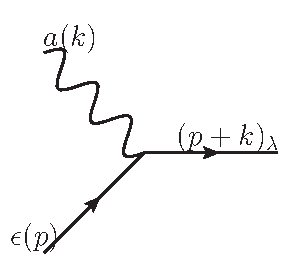
\includegraphics[scale=0.7]{eps/V-lambda} 
\end{minipage}
\hspace{8em}
$\overline{V}_\rho = $
\begin{minipage}{1in}
   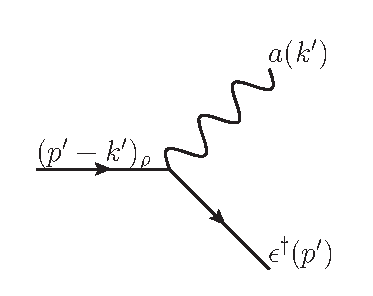
\includegraphics[scale=0.7]{eps/V-bar-rho} 
\end{minipage}



$U_\lambda = $
\begin{minipage}{1in}
   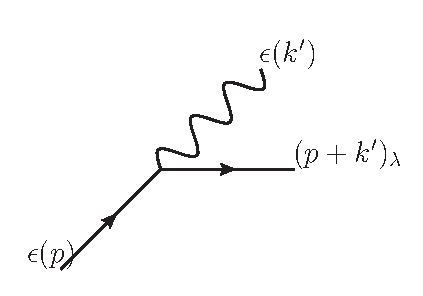
\includegraphics[scale=0.7]{eps/U-lambda} 
\end{minipage}
\hspace{8em}
$\overline{U}_\rho = $
\begin{minipage}{1in}
   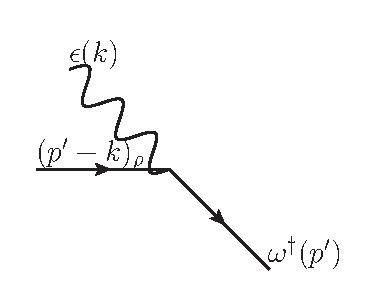
\includegraphics[scale=0.7]{eps/U-bar-rho} 
\end{minipage}

With the above definitions we see that the point-like interactions, taken from the two diagrams, will be

\begin{minipage}{1in}
   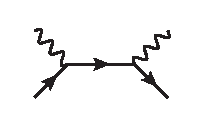
\includegraphics[scale=1]{eps/uncrossed-small} 
\end{minipage}
$ \to \overline{V}_\rho P^{\rho \lambda}(p+k) V_\lambda$
\hspace{5em}
\begin{minipage}{1in}
   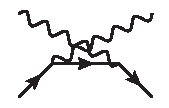
\includegraphics[scale=1]{eps/crossed-small} 
\end{minipage}
$ \to \overline{U}_\rho P^{\rho \lambda}(p+k') U_\lambda$



We only need terms one past leading order to find the $\v{S} \cdot \v{E} \times \v{A}$ term.  We'll tabulate the first two orders of each vertex for time and spatial components separately.  




The basic vertex inside $V_\lambda$ is, with incoming particle momentum $p^\mu$, incoming photon momentum $k^\alpha$ and outgoing $(p+k)^\lambda$:

\[
	ie[ g^{\mu\lambda}(2p + k)^\alpha - g^{\lambda \alpha} (p + [g]k)^\mu - g^{\alpha \mu} (p-[g-1]k)^\lambda ]
\]

Contracted with external charged particle and photon polarizations $\W_\mu$ and $\A_\alpha(k)$ we get:
\[
	V_\lambda = ie[\W^\lambda (2p + k) \cdot \A - \A^\lambda (p+[g]k) \cdot \W - \A \cdot \W (p-[g-1]k)^\lambda ]
\]
  
We can obtain the other three vertices simply by substituting the appropriate momenta and polarisations.  For instance, the similar vertex for outgoing momentum $(p+k)^\rho = (p' - k')^\rho$, photon $k'$, and final momentum $p'$ is

\[
	\overline{V}_\rho = ie[\W^{\dagger\rho} (2p' - k') \cdot \Adag - \A^\rho (p'-[g]k') \cdot \W^\dagger  - \Adag \cdot \W^\dagger  (p'+[g-1]k')^\rho ]
\]
We can obtain $\overline{V}_\rho$ just by substituting $\W^\dagger$ for $\W$, and $p'$ for $p$, and $-k'$ for $k$.  We'll only need to explicitly do the calculation for $V_\lambda$, since all four have the same form.



%%%%%%%%%%%%%%%%%%%%%%%%%%%%%%%%%%%%%%
\subsection{Calculation of $V_\lambda$}
We have chosen our gauge such that $\A_0=0$, which will help simplify the calculation.  We also only need the first two orders.

The leading order terms must have only the time-component of the charged particles momentum: the on mass-shell $p_0 = p'_0 \approx m$.  Corrections to $p_0$ do not enter at our level of approximation for the two photon diagrams. 

The next order terms have exactly one power of external momentum $\v{p}$ or photon momentum $\v{k}$, $\v{k'}$ or $k_0$, $k'_0$.  Any term containing $\W_0$ is of at least this order, since $\W^0(p) \approx \frac{\gv{\W} \cdot \v{p}}{m}$.

Anyway, now we'll calculate the terms explicitly.


\subsubsection{The $V_0$ term}
Consider first the time-component of $V$: 
$V_0 = ie[\W^0 (2p + k) \cdot \A - \A^0 (p+[g]k) \cdot \W - \A \cdot \W (p-[g-1]k)^0 ]$

%Term 1
Up to some outer factor the first term is then $\W^0 (2p + k) \cdot \A$.  Since $\W^0 =\frac{\gv{\W} \cdot \v{p}}{m}$ this becomes
\[
\W^0 (2p + k) \cdot \A = \frac{\gv{\W} \cdot \v{p}}{m} (2p + k) \cdot \A  = 2 \frac{\gv{\W} \cdot \v{p}}{m} p_0  \A_0 + \mathcal{O}(\frac{p^2}{m})
\]

The spatial component of $\A$ only appears with an additional power of momentum and so is too high order, and the $\A_0$ term vanishes in the chosen gauge.  So this term doesn't contribute at all to our result:
\[
\W^0 (2p + k) \cdot \A \sim \mathcal{O}(\frac{p^2}{m})
\]

%Term 2
The next term goes as $ -\A^0 (p+[g]k) \cdot \W$.   Obviously with our choice of gauge this doesn't contribute either.
% (Unneeded calculation in this gauge) Expanding the dot product we can use that $p \cdot \W = 0$ leaving only $k \cdot \W = -\v{k} \cdot \gv{\W}$.
%\[	-\A_0 (2k) \cdot \W = 2 \A_0 \v{k} \cdot \gv{\W} \]

%Term 3
The final term here is $- \A \cdot \W (p-[g-1]k)^0 $  Expanding the dot product and again using our choice of gauge we get
\[
	- \A \cdot \W (p-[g-1]k)^0   \approx - (\A_0 \W_0  - \v{\A} \cdot \gv{\W} ) (m - [g-1]k_0) = (m-[g-1]k_0)\v{\A} \cdot \gv{\W}
\]

%Sum
So the total from the $\lambda=0$ vertex is just 
\[
	V_0 = ie(m-[g-1]k_0)\v{\A} \cdot \gv{\W}
\]

\subsubsection{The $V_i$ term}
Now we look at the spatial component: $V_i = ie[\W^i (2p + k) \cdot \A - \A^i (p+[g]k) \cdot \W - \A \cdot \W (p-[g-1]k)^i ]$

% Term 1
In the first term we get simply
\[
	\W^i (2p + k) \cdot \A = \W^i ([2m + k_0]\A_0 - [2\v{p} + \v{k}] \cdot \v{\A} ]) 
\]

Which after applying the gauge conditions becomes
\[
	\W^i (2p + k) \cdot \A =  - 2 (\v{p} \cdot \v{\A} ) \W^i 
\]

%Term 2 \v{A} \cdot \gv{\W}	
For the second term $- \A^i (p+2k) \cdot \W$ we again use that $p \cdot \W=0$ so 
\[
	- \A^i (p+[g]k) \cdot \W \approx g \A^i \v{k} \cdot \gv{\W} 
\]
%Term 3
And in the third term $ - \A \cdot \W (p-[g-1]k)^i$ the $\A_0$ term is of too high order (irregardless of the gauge), leaving
\[
	- \A \cdot \W (p-[g-1]k)^i \approx \v{\A} \cdot \gv{\W} (p-[g-1]k)^i
\]	
All terms together give
\[
V_i = ie\left( [g]\v{k} \cdot \gv{\W} \A^i - 2\v{p} \cdot \v{\A} \W^i + \v{\A} \cdot \gv{\W} [p - [g-1]k]^i \right )
\]

\subsubsection{Tabulation}

We could (and I did) perform parallel calculations for the second vertex, but we can also note that it has exactly the same form, with the recipe being that $p \to p'$, $k \to -k'$, $\W \to \W^\dagger$.  Similar considerations work for $U$, where the only difference is that because of the crossed lines, we just swap $k$, $k'$.

So if we consider $V$ as a function of $p$, $k$ and $\W$: $V_\mu(p, k, \W)$ then 
\beqa
	\overline{V}_\mu &=& V_\mu(p', -k',  \W^\dagger)	\\
	U_\mu &=& V_\mu(p, k',  \W)			\\
	\overline{U}_\mu &=& V_\mu(p', -k, \W^\dagger)	\\
\eeqa





We want only the first two orders: write $X^{(1)}$ to indicate a leading order terms, $X^{(2)}$ to indicate next to leading order terms.

For the first vertex
\beqa
	V_0^{(1)} &=&	i e m \v{\A} \cdot \gv{\W}			\\
	V_0^{(2)} &=&	-i e [g-1] k_0  \v{\A} \cdot \gv{\W} 	\\
	V_i^{(1)} &=&	0				\\
	V_i^{(2)} &=&	 ie\left( [g]\v{k} \cdot \gv{\W} A^i - 2\v{p} \cdot \v{\A} \W^i + \v{\A} \cdot \gv{\W} [p - [g-1]k]^i \right )	\\
\eeqa

And for the second
\beqa
	\overline{V}_0^{(1)} &=&	i e m \v{\Adag} \cdot \gv{\W^\dagger}			\\
	\overline{V}_0^{(2)} &=&	i e [g-1] k'_0 \v{\Adag} \cdot \gv{\W^\dagger}			\\
	\overline{V}_i^{(1)} &=&	0								\\
	\overline{V}_i^{(2)} &=&	i e ( -[g]\v{k'} \cdot \gv{\W^\dagger} {\Adag}^i - 2\v{p'} \cdot \v{\Adag} \W^{\dagger^i}
				+ \v{\Adag} \cdot \gv{\W^\dagger} [p' + [g-1]k']^i )	\\
\eeqa

Using $U$ to denote the vertices of the crossed diagram.

\beqa
	U_0^{(1)} &=&	i e m \v{\Adag} \cdot \gv{\W}			\\
	U_0^{(2)} &=&	-i e [g-1] k'_0  \v{\Adag} \cdot \gv{\W} 	\\
	U_i^{(1)} &=&	0				\\
	U_i^{(2)} &=&	 i e \left( [g]\v{k'} \cdot \gv{\W} \Adag^i - 2\v{p} \cdot \v{\Adag} \W^i + \v{\Adag} \cdot \gv{\W} [p - [g-1]k']^i \right )	\\
\eeqa

And for the second
\beqa
	\overline{U}_{0}^{(1)} &=&	i e m \v{\A} \cdot \gv{\W^\dagger}			\\
	\overline{U}_{0}^{(2)} &=&	i e [g-1] k_0 \v{\A} \cdot \gv{\W^\dagger}			\\
	\overline{U}_{i}^{(1)} &=&	0								\\
	\overline{U}_{i}^{(2)} &=&	i e ( -[g]\v{k} \cdot \gv{\W^\dagger} {\A}^i - 2\v{p'} \cdot \v{\A} \W^{\dagger^i}
				+ \v{\A} \cdot \gv{\W^\dagger} [p' + [g-1]k]^i )	\\
\eeqa
We also write again the possibly relevant propagator terms $P^{\lambda \rho}(q)$.
\beqa
 P^{00} &=& \frac{i}{m^2} 	\\
 P^{0i} &=& P^{i0} = i\frac{  q^i  }{4m^3}		\\
 P^{ij} &=& - \left(1 - \frac{q_0 - m}{2m} \right )\frac{i \delta^{ij} }{4m^2} 	
\eeqa
Where $q = p+k$ for the uncrossed diagrams, and $q = p+k'$ for crossed.  For our particular result only $P_{00}$ will contribute, though.  And since at the needed order only the pure contact term contributes, the momentum dependence of the propagator doesn't show up in the final result.

 
From the above pieces we can calculate the point-like terms which arise from the two-vertex diagram.  Including both crossed and uncrossed diagrams:

\begin{minipage}{1in}
   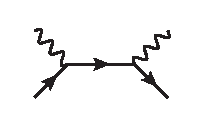
\includegraphics[scale=1]{eps/uncrossed-small} 
\end{minipage}
\hspace{1em}$+$
\begin{minipage}{1in}
   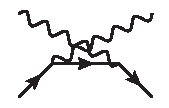
\includegraphics[scale=1]{eps/crossed-small} 
\end{minipage}
$
	\to \overline{V}_\rho P^{ \rho \lambda}(p+k) V_\lambda +   \overline{U}_\rho P^{ \rho \lambda}(p+k') U_\lambda
$

\subsection{Two vertex contribution}

We can now calculate relevant contributions to the scattering amplitude from the two vertex diagrams.
\subsubsection{Leading order}
The leading order term from uncrossed diagrams will be $V_\lambda^{(1)} P^{\lambda \rho} \overline{V}_\rho^{(1)}$, or
\beqa
V_{\lambda=0}^{(1)} P^{00} \overline{V}_{0}^{(1)} + V_{i}^{(1)} P^{ij} \overline{V}_{j}^{(1)}	
	&=&	-e^2 m^2 \gv{\W^\dagger} \cdot \v{\Adag} \frac{i}{m^2}\v{\A} \cdot \gv{\W} + 0 	\\
	&=& -i e^2  (\gv{\W^\dagger} \cdot \v{\Adag} ) ( \v{\A} \cdot \gv{\W})  \\
\eeqa
From crossed diagrams
\beqa
U_{0}^{(1)} P^{00} \overline{U}_{0}^{(1)} + U_{i}^{(1)} P^{ij} \overline{U}_{j}^{(1)}	
	&=& - i e^2 (\gv{\W^\dagger} \cdot \v{\A} ) ( \v{\Adag} \cdot \gv{\W} ) \\
\eeqa

So the total contribution is
\[
- i e^2 (\gv{\W^\dagger} \cdot \v{\A}) ( \v{\Adag} \cdot \gv{\W}) - i e^2 (\gv{\W^\dagger} \cdot \v{\Adag}) ( \v{\A} \cdot \gv{\W})
\]

\subsubsection{Contributions to $\v{E} \times \v{A}$ terms}
The particular coefficient we care about in the NRQED Lagrangian contains $k_0 \v{A}(k)$.

Looking at the above list we see only the second order terms $V^{(2)}_0$ will contribute to this coefficient.
\[
V_{\lambda=0}^{(1)} P^{00} \overline{V}_{\rho=0}^{(2)} + V_{\lambda=2}^{(1)} P^{00} \overline{V}_{\rho=0}^{(1)}	
\]
This is
\[
- e^2 \left(  [m \v{\A} \cdot \gv{\W} ] \frac{i}{m^2} [(g-1)k'_0 \v{\Adag} \cdot \gv{\W^\dagger} ] -  [ (g-1)k_0  \v{\A} \cdot \gv{\W} ]\frac{i}{m^2} [m \v{\Adag} \cdot \gv{\W^\dagger}] \right )
	=
- i e^2 (g-1)\frac{ k'_0 - k_0}{m}  [\v{\Adag} \cdot \gv{\W^\dagger}] [\v{\A} \cdot \gv{\W} ]
\]



The contribution from the crossed diagrams is
\[
U_{\lambda=0}^{(1)} P^{00} \overline{U}_{\rho=0}^{(2)} + U_{\lambda=2}^{(1)} P^{00} \overline{U}_{\rho=0}^{(1)}	
\]

\[
=- e^2 \left(  [m \v{\Adag} \cdot \gv{\W} ] \frac{i}{m^2} [(g-1)k_0 \v{\A} \cdot \gv{\W^\dagger} ] -  [ (g-1)k'_0  \v{\Adag} \cdot \gv{\W} ]\frac{i}{m^2} [m \v{\A} \cdot \gv{\W^\dagger}] \right )
	=
- i e^2 (g-1)\frac{ k_0 - k'_0}{m} [\v{\A} \cdot \gv{\W^\dagger}] [\v{\Adag} \cdot \gv{\W} ]
\]

So the total contribution is
\[
	-ie^2 (g-1) \frac{ k_0 - k'_0}{m} \left( [\v{\A} \cdot \gv{\W^\dagger}] [\v{\Adag} \cdot \gv{\W} ] -  [\v{\Adag} \cdot \gv{\W^\dagger}] [\v{\A} \cdot \gv{\W} ] \right )
\]




We can put this in the form of a matrix element using the previously derived identity
\[(\v{W^\dagger} \cdot \v{v} )( \v{u} \cdot \v{W} )= W^\dagger_a \left[ \v{u} \cdot \v{v} \delta_{ab} - (\v{S}_{ac} \cdot \v{u})(\v{S}_{cb} \cdot \v{v}) \right ] W_b\] 


Understanding that the wave functions $\W$ are contracted only with the spin structure, we write now
\[
		  -i (g-1)e^2  \frac{ k_0 - k'_0}{m} \W^\dagger \left( \v{\Adag} \cdot \v{\A} - (\v{S} \cdot \v{\Adag}) (\v{S} \cdot \v{\A})  -\v{\A} \cdot \v{\Adag} + \v{S} \cdot \v{\A} \v{S} \cdot \v{\Adag} \right ) \W
\]
Which after simplification is
\[
	-i  e^2 (g-1) \frac{ k_0 - k'_0}{m} \W^\dagger \left(  [\v{S} \cdot \v{\A}, \v{S} \cdot \v{\Adag}] \right ) \W
=
	e^2 (g-1) \frac{ k_0 - k'_0}{m} \W^\dagger  \left( \v{S} \cdot \v{\A} \times \v{\Adag} \right ) \W
\]



%%%%%%%%%%%%%%%%%%%% SUM OF two-photon vertex and two one-photon vertices   %%%%%%%%%%%%%%%%%%%%%%%%5
\section{Sum of two-photon vertex and two-vertex tree diagrams}
Now we'll find the total scattering amplitude to the order we need.  (One power of $\frac{p}{m}$ past leading order.) 

First consider just the leading order terms.  The contribution from the fundamental two-photon vertex is:
\[
-2 i e^2\gv{\W^\dagger} \cdot \gv{\W} \v{\Adag} \cdot \v{\A}  
+ i e^2(\gv{\W^\dagger} \cdot  \v{\A}) (\v{\Adag} \cdot \gv{\W})	
+ i e^2(\gv{\W^\dagger} \cdot  \v{\Adag}) (\v{\A} \cdot \gv{\W})	
\]

The contribution from leading order contact terms of the two-vertex diagrams is:
\[
- i e^2 (\gv{\W^\dagger} \cdot \v{\A}) ( \v{\Adag} \cdot \gv{\W}) - i e^2 (\gv{\W^\dagger} \cdot \v{\Adag}) ( \v{\A} \cdot \gv{\W}) 
\]
The sum of leading order contributions to the scattering is then just 
\[
- 2 i e^2\gv{\W^\dagger} \cdot \gv{\W} \v{\Adag} \cdot \v{\A}  
\]

which in terms of the spinors $\phi$ would be
\[
 - i\frac{e^2}{m} \phi^\dagger (\v{\A}\cdot \v{\Adag} ) \phi
\]


Then consider terms which implicitly will fix $\v{E}$.  The fundamental vertex contains no terms with $\v{E}$ in them, so the only term is from the two-vertex diagrams:
\[
 e^2 (g-1) \frac{ k_0 - k'_0}{m} \W^\dagger  \left( \v{S} \cdot \v{\A} \times \v{\Adag} \right ) \W
\]
Which in terms of $\phi$ is just
\[
 \frac{e^2}{2m^2} (g-1) ( k_0 - k'_0 ) \phi^\dagger  \left( \v{S} \cdot \v{\A} \times \v{\Adag} \right ) \phi
\]





\section{NRQED Lagrangian}



%full lagrangian
We have used the relativistic theory to calculate two processes.  Now we will calculate these same scattering amplitudes from the NRQED Lagrangian, and thus fix its coefficients.

We write the NRQED Lagrangian in terms of gauge invariant quantities $\v{E}$, $\v{B} $ and $\v{D} = \grad - ie\v{A}$ To the order we care about it is:
\scriptsize
\beqa
	\mathcal{L}_{NRQED} &=& \Psi^\dagger \{ i(\partial_0 + ieA_0) + \frac{\v{D}^2}{2m} + \frac{\v{D}^4}{8m^3} 
		+ c_F e \frac{\v{S} \smalldot \v{B}} {2m}   	
		+ c_D \frac{ e(\v{D} \smalldot \v{E} - \v{E} \smalldot \v{D} ) }{8m^2}	
		+ c_Q \frac{e Q_{ij} (D_i E_j - E_i D_j) }{8m^2}	
	\\&&	+ c_S \frac{ ie \v{S} \smalldot ( \v{D} \times \v{E} - \v{E} \times \v{D} )}{8m^2}
		+ c_{W_1} \frac{ e [ \v{D}^2 (\v{S} \smalldot \v{B} ) + (\v{S} \smalldot \v{B} ) \v{D}^2] }{8m^3}	
		- c_{W_2} \frac{ e D^i (\v{S} \smalldot \v{B} ) D^i }{4m^3}
		+ c_{p'p} \frac{ e [ (\v{S} \smalldot \v{D}) (\v{B} \smalldot \v{D}) + (\v{B} \smalldot \v{D})(\v{S} \smalldot \v{D}) }{8m^3} \} \Psi
\eeqa
\normalsize
To fix the coefficients we calculate two processes.  First, to fix the terms with one power of $A$, we calculate elastic scattering off an external field.  Second, to fix the terms with two powers of the field $A$, we calculate Compton scattering.

%NOTE we use D = \partial - ieA
\subsection{Scattering off external field in NRQED}
We can write down those terms in the NRQED Lagrangian which have one power of the external field.  This set of terms will not, by themselves, be gauge invariant. If, for example, a coefficient exists before a term with both one and two powers of $A$, we'll want to make sure we get the same result in both calculations.  We'll add a superscript to the coefficient to keep track of this: so below we write $c^1_S$.

In writing the expansion of terms like $\v{D}^4$ it is convenient to use anticommutators.
\small
\beqa
\mathcal{L}_A &=& \Psi^\dagger (  -eA_0- ie  \frac{ \{\nabla_i, A_i \} }{2m} -ie \frac{ \{\grad^2, \{\nabla_i, A_i \}  \} }{8m^3} 
		+ c_F e \frac{\v{S} \smalldot \v{B}} {2m}   	
		+ c_D \frac{ e(\v{\grad} \smalldot \v{E} - \v{E} \smalldot \v{\grad} ) }{8m^2}	
		+ c_Q \frac{e Q_{ij} (\nabla_i E_j - E_i \nabla_j) }{8m^2}	
	\\&&	+ c^{1}_S \frac{ ie \v{S} \smalldot ( \v{\grad} \times \v{E} - \v{E} \times \v{\grad} )}{8m^2}
		+ c_{W_1} \frac{ e [ \v{\grad}^2 (\v{S} \smalldot \v{B} ) + (\v{S} \smalldot \v{B} ) \v{\grad}^2] }{8m^3}	
		- c_{W_2} \frac{ e \nabla^i (\v{S} \smalldot \v{B} ) \nabla^i }{4m^3}
		+ c_{p'p} \frac{ e [ (\v{S} \smalldot \v{\grad}) (\v{B} \smalldot \v{\grad}) + (\v{B} \smalldot \v{\grad})(\v{S} \smalldot \v{\grad}) }{8m^3} \big )\Psi
\eeqa
\normalsize


We want to calculate from this a particular process: scattering off an external field, with incoming momentum $\v{p}$, outgoing $\v{p'}$, and $\v{q} = \v{p'} - \v{p}$.  There is one diagram associated with each term above, but the total amplitude is just going to be the sum of all these one-photon vertices.  These of course can just be read off directly from the Lagrangian: we replace the fields $\Psi$ with the spinors $\phi$, and any operator $\grad$ acting will become $i\v{p}$ if it acts on the right, $i\v{p'}$ if it is to the left.

We can simplify some expressions involving $\grad$ and $\v{E}$:
Because $Q_{ij}$ is symmetric:
\[
	 Q_{ij} (\nabla_i E_j - E_i \nabla_j ) = Q_{ij} [\nabla_i, E_j] = Q_{ij} (\partial_i E_j)
\]

And because $E_i = -\partial_i \Phi$
\[
	\v{\grad} \times \v{E} - \v{E} \times \v{\grad} =  - 2 \v{E} \times \v{\grad}
\]
And also use that
\[
\v{\grad} \smalldot \v{E} - \v{E} \smalldot \v{\grad} = (\partial_i E_i)
\]


Now we can write down the scattering amplitude for scattering off the external field, before we apply any assumptions about the particular process.
\beqa
	iM &=&
		ie\phi^\dagger \Bigg( - A_0 +    \frac{ \v{A} \cdot (\v{p} + \v{p'}) }{2m} 
		- \frac{  \v{A} \cdot (\v{p} + \v{p'}) \v{p}^2 + \v{p'}^2 \v{A} \cdot (\v{p} + \v{p'}) }{8m^3} 
	\\&&	+ c_F  \frac{\v{S} \smalldot \v{B}} {2m}   	
		+ c_D \frac{ ( \partial_i E_i ) }{8m^2}	
		+ c_Q \frac{Q_{ij}  ( \partial_i E_j ) }{8m^2}	
		+ c^{1}_S \frac{  \v{E} \times \v{p} }{4m^2}
	\\&&	- c_{W_1}  \frac{  (\v{S} \smalldot \v{B} ) (\v{p}^2 + \v{p'}^2)  }{8m^3}
		+ c_{W_2} \frac{  (\v{S} \smalldot \v{B} ) (\v{p} \cdot \v{p'}) }{4m^3}
		-  c_{p'p} \frac{  (\v{S} \smalldot \v{p'}) (\v{B} \smalldot \v{p}) + (\v{B} \smalldot \v{p'}) (\v{S} \smalldot \v{p}) }{8m^3} \Bigg )\phi
\eeqa

The above can be simplified somewhat.  We choose our gauge such that $\nabla_i A_i = 0$.  If we specify elastic scattering then kinematics dictate that $\v{p'}^2 = \v{p}^2$.   Finally, if we consider $\v{B}$ constant, the $c_W$ terms become indistinguishable, since $[ \nabla_i, B_j] = 0$.    (It is only this last assumption that costs us any information.)  Then the scattering amplitude, as calculated from $\mathcal{L}_{NRQED}$, is:

\beqa
	iM &=&
		ie\phi^\dagger \Bigg(  -A_0 +  \frac{ \v{A} \cdot \v{p} }{m} - \frac{  (\v{A} \cdot \v{p}) \v{p}^2   }{2m^3} 
		+ c_F  \frac{\v{S} \smalldot \v{B}} {2m}   	
		+ c_D \frac{ ( \partial_i E_i ) }{8m^2}	
		+ c_Q \frac{ Q_{ij} ( \partial_i E_j ) }{8m^2}	
	\\&&	+ c^{1}_S \frac{  \v{E} \times \v{p} }{4m^2}
		- (c_{W_1} -c_{W_2}) \frac{   (\v{S} \smalldot \v{B} ) \v{p}^2  }{4m^3}	
		-  c_{p'p} \frac{   (\v{S} \smalldot \v{p}) (\v{B} \smalldot \v{p})  }{4m^3} \Bigg )\phi
\eeqa

\subsection{Comparison with relativistic result}

Having calculated the same process in both the relativistic theory and in our NRQED effective theory, we can compare the two amplitudes and fix the coefficients.

The NRQED amplitude is 
\beqa
	iM &=&
		ie\phi^\dagger \Bigg( - A_0 +   \frac{ \v{A} \cdot \v{p} }{m} - \frac{  (\v{A} \cdot \v{p}) \v{p}^2   }{2m^3} 
		+ c_F  \frac{\v{S} \smalldot \v{B}} {2m}   	
		+ c_D \frac{ ( \partial_i E_i ) }{8m^2}	
		+ c_Q \frac{ Q_{ij} ( \partial_i E_j ) }{8m^2}	
	\\&&	+ c^{1}_S \frac{  \v{E} \times \v{p} }{4m^2}
		- (c_{W_1} -c_{W_2}) \frac{   (\v{S} \smalldot \v{B} ) \v{p}^2  }{4m^3}	
		-  c_{p'p} \frac{   (\v{S} \smalldot \v{p}) (\v{B} \smalldot \v{p})  }{4m^3} \Bigg )\phi
\eeqa


While the relativistic amplitude was
\[
iM_{REL} = -ie \phi^\dagger \Big (
		 A_0  - \frac{\v{p}\cdot \v{A} }{m} + \frac{\v{p}\cdot \v{A} \v{p}^2}{2m^3}
		- \frac{g-1}{2m^3}\{ \grad \cdot \v{E} -  \v{S} \cdot \v{p} \times \v{E} - S_i S_j \grad_i E_j \}
		- g\frac{1}{2m} \v{S} \cdot \v{B}
		+ \v{S} \cdot \v{B} \frac{\v{p}^2}{2m^3}
		+ \frac{g-2}{4m^3}(\v{S} \cdot \v{p} )( \v{B} \cdot \v{p})
	\Big ) \phi
\]


We should rewrite term $\grad \cdot \v{E}  - S_i S_j \grad_i E_j$ using the quadropole moment tensor $Q_{ij} = \frac{1}{2} ( S_i S_j + S_j S_i - \frac{2}{3}\v{S}^2 )$.

Remember that $\nabla_i E_j$ is actually symmetric under exchange of $i$ and $j$.  Then we can write
\[
	S_i S_j \nabla_i E_j = \frac{1}{2} (S_i S_j + S_j S_i) = (Q_{ij} + \frac{1}{3} \v{S}^2 \delta_{ij}) \nabla_i E_j
\]
\[
	= Q_ij \nabla_i E_j + \frac{2}{3} \grad \cdot \v{E}
\]
Written using this identity, the relativistic amplitude is
\[
iM_{REL} = -ie \phi^\dagger \Big (
		 A_0  - \frac{\v{p}\cdot \v{A} }{m} + \frac{\v{p}\cdot \v{A} \v{p}^2}{2m^3}
		- \frac{g-1}{2m^3}\{ \frac{1}{3}\grad \cdot \v{E} -  \v{S} \cdot \v{p} \times \v{E} - Q_{ij} \grad_i E_j \}
		- g\frac{1}{2m} \v{S} \cdot \v{B}
		+ \v{S} \cdot \v{B} \frac{\v{p}^2}{2m^3}
		+ \frac{g-2}{4m^3}(\v{S} \cdot \v{p} )( \v{B} \cdot \v{p})
	\Big ) \phi
\]

Comparing the two, the coefficients are:
\beqa
	c_F &=& g \\
	c_D &=&	\frac{4(g-1)}{3}	\\
	c_Q &=&	-4(g-1)	\\
	c^1_S &=& 2 (g-1)	\\
	(c_{W_1} - c_{W_2}) &=&	2	\\
	c_{p'p}	&=& (g-2)		\\
\eeqa



%%%%%%%%%%%%%%%%%%%%%%%%%%%%%
% TWO PHOTON
%%%%%%%%%%%%%%%%%%%%%%%%%%%%%%

%Two photon lagrangian
\subsection{Two photon scattering in NRQED}


We want to calculate the Compton scattering in the nonrelativistic theory.  We choose the gauge such that the photon polarisations obey $\A_0 = 0$.  In general we should consider both terms arising from two-photon vertices, and those from tree level diagrams of two one-photon vertices.  However, because of the approach we take in calculating the process from the relativistic Lagrangian, we only need the former terms.

Further, ultimately we only care about a few of these terms, ignoring terms which have both $\v{B}$ and $\v{A}$.

Note that both $(\v{A} \smalldot \v{E} - \v{E} \smalldot \v{A} )=0$ and $Q_{ij} (A_i E_j - E_i A_j) = 0$ by symmetry.

The remaining terms we're interested in are:
\scriptsize
\beqa
	\mathcal{L}_{A^2} &=& \Psi^\dagger ( - \frac{e^2 \v{A}^2}{2m}  - e^2 \frac{ \{ \grad^2, \v{A}^2 \} 
}{8m^3} - e^2\frac{ \{\nabla_i, A_i \} \{\nabla_j, A_j\} }{8m^3}
		+ c^2_S \frac{ e^2 \v{S} \smalldot ( \v{A} \times \v{E} - \v{E} \times \v{A} )}{8m^2} ) \Psi
\eeqa
\normalsize

If we want the scattering amplitude, we replace $\Psi$ with $\phi$, and contract $\v{A}$ with photon polarisations $\A$ and $\Adag$.  In the gauge chosen, $\v{E}(k) = -\partial_0 \v{\A} = i k_0 \v{\A}(k)$.

Contracted with the photon of mometum $k$ we get $\v{E} \to i k_0 \v{\A}$, while with the photon of momentum $k'$ we have $\v{E} \to i k'_0 \v{\Adag}$.  So:
\[
	\v{A} \times \v{E} = - \v{A} \times (\partial_0 \v{A})
		\to 
	-i(k_0' \v{\A} \times \v{\Adag} + k_0 \v{\Adag} \times \v{\A} ) = i ( k_0' - k_0) \v{\A} \times \v{\Adag}
\]
And
\[
	\v{E} \times \v{A} = - (\partial_0 \v{A}) \times  \v{A}
		\to 
	-i( k_0 \v{\A} \times \v{\Adag} + k_0' \v{\Adag} \times \v{\A} ) = -i ( k_0' - k_0) \v{\A} \times \v{\Adag}
\]
So from the term in the Lagrangian 
\[
 c^2_S \Psi^\dagger \frac{ e^2 \v{S} \smalldot ( \v{A} \times \v{E} - \v{E} \times \v{A} )}{8m^2} ) \Psi
\]
we get in the scattering amplitude

\[
  -i c^2_S \phi^\dagger  \Big ( \frac{e^2}{4m^2}    i(k_0 - k_0')    \v{\A} \times \v{\Adag} \Big ) \phi
	=
     c^2_S \frac{e^2}{4m^2} \phi^\dagger  \Big ( (k_0 - k_0')    \v{\A} \times \v{\Adag} \Big ) \phi
\]

\subsection{Comparison with relativistic result}
From the relativistic theory, we calculated the scattering amplitude of the same process:
\[
iM_{REL} = 
 \frac{e^2}{2m^2} (g-1) ( k_0 - k'_0 ) \phi^\dagger  \left( \v{S} \cdot \v{\A} \times \v{\Adag} \right ) \phi
\]


So comparing the two results, we can fix the coefficient.
\[
	c^2_s = 2(g-1)
\]



\subsection{Final Lagrangian}
Now we can write down what the NRQED Lagrangian looks like (for constant $\v{B}$.)


%lagragnian
\small
\beqa
	\mathcal{L}_{NRQED} &=& \Psi^\dagger \{ i(\partial_0 + ieA_0) + \frac{\v{D}^2}{2m} + \frac{\v{D}^4}{8m^3} 
		+ e g  \frac{\v{S} \smalldot \v{B}} {2m}   	
		+ e(g-1)\frac{ ( \partial_i E_i ) }{6m^2}	
		- e(g-1) \frac{ Q_{ij} ( \partial_i E_j ) }{2m^2}	
	\\&&	+(g-1) \frac{ ie \v{S} \smalldot ( \v{D} \times \v{E} - \v{E} \times \v{D} )}{4m^2}
		- e\frac{   (\v{S} \smalldot \v{B} ) \v{p}^2  }{2m^3}	
		+(g-2) \frac{ e  (\v{S} \smalldot \v{D}) (\v{B} \smalldot \v{D})  }{4m^3} \} \Psi
\eeqa
\normalsize


\subsubsection{Hamiltonian}
Or if we write the Hamiltonian instead (using $\v{D} = i (\v{p} - e \v{A})$)

\small
\beqa
	\mathcal{H}_{NRQED} &=& \Psi^\dagger \{  \frac{(\v{p}-e\v{A})^2}{2m} - \frac{(\v{p}-e\v{A})^4}{8m^3}
		 + eA_0 
		- e g  \frac{\v{S} \smalldot \v{B}} {2m}   	
		- e(g-1)\frac{ ( \partial_i E_i ) }{6m^2}	
		+ e(g-1) \frac{ Q_{ij} ( \partial_i E_j ) }{2m^2}	
	\\&&	+(g-1) \frac{ e \v{S} \smalldot ( \v{p} \times \v{E} - \v{E} \times \v{p} )}{4m^2}
		-(g-1) \frac{ e^2 \v{S} \smalldot  \v{A} \times \v{E} }{2m^2}
		+ e\frac{   (\v{S} \smalldot \v{B} ) \v{p}^2  }{2m^3}	
		+(g-2) \frac{ e  (\v{S} \smalldot \v{p}) (\v{B} \smalldot \v{p})  }{4m^3} \} \Psi
\eeqa
\normalsize


 
\appendix



\section{Spin identity}
The product of two spin-1 matrices is

Our representation defines the spin matrices as follows:
$${(S_k)}_{ij}=-i \epsilon_{ijk}$$



The product of two such spin matrices is given by:
\begin{eqnarray*}
{(S_k S_\ell)}_{ij} 
	& = & {(S_k)}_{ia} {(S_\ell)}_{aj} \\
	& = & -\epsilon_{iak} \epsilon_{aj\ell} \\
	& = & (\delta_{k\ell} \delta_{ij} - \delta_{kj} \delta_{\ell i} )
\end{eqnarray*}

We can use this to write some pair of vector components $u_i v_j$ as a matrix structure.  Contract both sides of the above identity with $v_k$ and $u_\ell$.  The result is
\[
	[(\v{S} \cdot \v{v} )(\v{S} \cdot \v{u})]_{ij}
		= \v{u} \cdot \v{v} \delta_{ij} - u_i v_j 
\]
or equivalently
\[
	u_i v_j = \v{u} \cdot \v{v} \delta_{ij}  - [(\v{S} \cdot \v{v} )(\v{S} \cdot \v{u})]_{ij}
\]
The indices on the second term on the write refer to the indices of the product of spin matrices.  We will use this identity frequently in the following form:
\[
	(\v{W^\dagger} \cdot \v{v} )( \v{u} \cdot \v{W} )
		=	\v{W^\dagger} \left[ \v{u} \cdot \v{v} - (\v{S} \cdot \v{u} )(\v{S} \cdot \v{v}) \right ] \v{W}
\]
(Note that the vector dotted into $W^\dagger$ appears dotted with right-most spin matrix.)


\section{Anticommutator identity}
\begin{eqnarray*}
\left \{ \frac{\v{p}^2}{2} - (\v{S} \cdot \v{p})^2, \v{S} \cdot \v{B} \right \}
	&=&	 \v{p}^2 \v{S} \cdot \v{B} - [(\v{S} \cdot \v{p})^2 \v{S} \cdot \v{B} + \v{S} \cdot \v{B} (\v{S} \cdot \v{p})^2  ]	\\
	&=&	 \v{p}^2 \v{S} \cdot \v{B} - (S_i S_j S_k + S_k S_j S_i) p_i p_j B_k
\end{eqnarray*}

To simplify that triple product of spin matrices, we can use their explicit form:
\begin{eqnarray*}
	(S_i S_j S_k )_{ab}
		&=&	i\epsilon_{aci}\epsilon_{cdj}\epsilon_{dbk}	\\
		&=&	i(\delta_{id} \delta_{aj} - \delta_{ij} \delta_{ad})\epsilon_{dbk}	\\
		&=&	i(\delta_{aj} \epsilon_{ibk} - \delta_{ij} \epsilon_{abk})		\\
	(S_i S_j S_k + S_k S_j S_i)_{ab}
		&=& i(\delta_aj \epsilon_{ibk} + \delta_{aj} \epsilon_{kbi} -\delta_{ij} \epsilon_{abk} -\delta{kj}\epsilon_{abi})	\\
		&=& -i(\delta_{ij} \epsilon_{abk} + \delta_{kj} \epsilon_{abi})	\\
		&=&	\delta_{ij} {(S_k)}_{ab} + \delta_{kj} {(S_i)}_{ab}	
\end{eqnarray*}
Now 
\begin{eqnarray*}
 \v{p}^2 \v{S} \cdot \v{B} - (S_i S_j S_k + S_k S_j S_i) p_i p_j B_k
 	&=& \v{p}^2 \v{S} \cdot \v{B} - (\delta_{ij} S_k + \delta_{kj} S_i	) p_i p_j B_k	\\
 	&=& - (\v{S} \cdot \v{p}) (\v{B} \cdot \v{p})
\end{eqnarray*}





